% Digital Logic Report Template
% Created: 2020-01-10, John Miller

%==========================================================
%=========== Document Setup  ==============================

% Formatting defined by class file
\documentclass[11pt]{article}

% ---- Document formatting ----
\usepackage[margin=1in]{geometry}	% Narrower margins
\usepackage{booktabs}				% Nice formatting of tables
\usepackage{graphicx}				% Ability to include graphics

%\setlength\parindent{0pt}	% Do not indent first line of paragraphs 
\usepackage[parfill]{parskip}		% Line space b/w paragraphs
%	parfill option prevents last line of pgrph from being fully justified

% Parskip package adds too much space around titles, fix with this
\RequirePackage{titlesec}
\titlespacing\section{0pt}{8pt plus 4pt minus 2pt}{3pt plus 2pt minus 2pt}
\titlespacing\subsection{0pt}{4pt plus 4pt minus 2pt}{-2pt plus 2pt minus 2pt}
\titlespacing\subsubsection{0pt}{2pt plus 4pt minus 2pt}{-6pt plus 2pt minus 2pt}

% ---- Hyperlinks ----
\usepackage[colorlinks=true,urlcolor=blue]{hyperref}	% For URL's. Automatically links internal references.

% ---- Code listings ----
\usepackage{listings} 					% Nice code layout and inclusion
\usepackage[usenames,dvipsnames]{xcolor}	% Colors (needs to be defined before using colors)

% Define custom colors for listings
\definecolor{listinggray}{gray}{0.98}		% Listings background color
\definecolor{rulegray}{gray}{0.7}			% Listings rule/frame color

% Style for Verilog
\lstdefinestyle{Verilog}{
	language=Verilog,					% Verilog
	backgroundcolor=\color{listinggray},	% light gray background
	rulecolor=\color{blue}, 			% blue frame lines
	frame=tb,							% lines above & below
	linewidth=\columnwidth, 			% set line width
	basicstyle=\small\ttfamily,	% basic font style that is used for the code	
	breaklines=true, 					% allow breaking across columns/pages
	tabsize=3,							% set tab size
	commentstyle=\color{gray},	% comments in italic 
	stringstyle=\upshape,				% strings are printed in normal font
	showspaces=false,					% don't underscore spaces
}

% How to use: \Verilog[listing_options]{file}
\newcommand{\Verilog}[2][]{%
	\lstinputlisting[style=Verilog,#1]{#2}
}




%======================================================
%=========== Body  ====================================
\begin{document}

\title{ELC 2137 Lab 06: MUX and 7-segment Decoder}
\author{Yiting Wang}

\maketitle


\section*{Summary}

In this lab, we will be setting up a circuit to display an 8-bit number on two 7-segment displays (i.e.two  hexadecimal  digits). And we will design a couple of combinational logic modules in Verilog and then implement your design on an FPGA. After completing this lab, we should be able to write a multiplexer in Verilog using the conditional operator, Write combinational Verilog components using an always block, Define and use multi-bit signals (vectors), Instantiate and connect components in a top-level module, Use provided constraint files to specify package pins, and Implement design on FPGA (Digilent Basys3 board).\\



\section*{Q\&A}

\begin{enumerate}
	\item List of errors found during simulation. What does this tell you about why we run simulations?\\
	
	When I ran the Simulation, Synthesis and Implementation, there isn't any errors only a warning. I do made some mistakes about my code. \\
	After I ran the Simulation, I found the results is not match with my  expected results table, so I found some mistakes about my code.\\
	\item How many wires are connected to the 7-segment display? If the segments were not all connected together, how many wires would there have to be? Why do we prefer the current method  vs. separating all of the segments?\\
	
	How many wires are connected to the 7-segment display? 2. One input for num, and one output for sseg.\\ 
	If the segments were not all connected together, how many wires would there have to be? 11. \\
	Why do we prefer the current method  vs. separating all of the segments? because when we do some bigger project in the future, we will have more inputs and outputs, if we use the current method, it will help us to organize them easier.\\
\end{enumerate}



\section*{Results}	

	Firgure 1 is the simulation waveform and ERT of the 4-bit Multiplexer.
	\begin{figure}[ht]\centering
		\begin{tabular}{l|rrrr}
			Time (ns): & 0 & 10 & 20 & 30 \\
			\midrule
			in1 & 1111 & 1111 & 0100 & 0100 \\
			in0 & 0000 & 0000 & 1101 & 1101 \\
			sel & 0 & 1 & 0 & 1 \\
			\midrule
			out & 0000 & 1111 & 1101 & 0100 \\
			\bottomrule
		\end{tabular}\medskip
		
		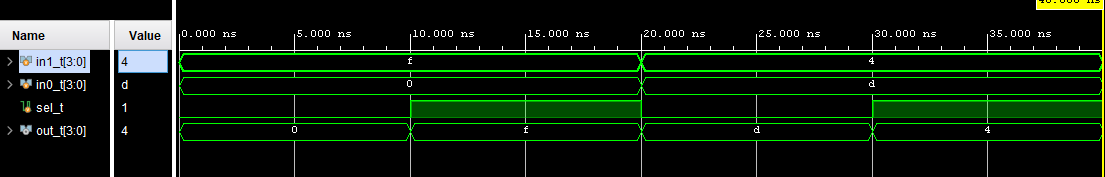
\includegraphics[width=1\textwidth]{mux2_4b_simulation}
		\caption{the simulation waveform and ERT of the 4-bit Multiplexer}
		\label{fig:mux2_4b_simulation}
	\end{figure}
	
	Firgure 2 is the simulation waveform and ERT of the Seven-segment Decoder.
	\begin{figure}[ht]\centering
		\begin{tabular}{l|rrrr|rrrr|rrrr|rrrr}
			Time (ns): & 0 & 10 & 20 & 30 & 40 & 50 & 60 & 70 & 80 & 90 & 100 & 110 & 120 & 130 & 140 & 150 \\
			\midrule
			num (hex) & 0 & 1 & 2 & 3 & 4 & 5 & 6 & 7 & 8 & 9 & a & b & c & d & e & f \\
			\midrule
			sseg (hex) & 40 & 79 & 24 & 30 & 19 & 12 & 02 & 78 & 00 & 18 & 08 & 03 & 46 & 21 & 06 & 0e \\
			\bottomrule
		\end{tabular}\medskip
		
		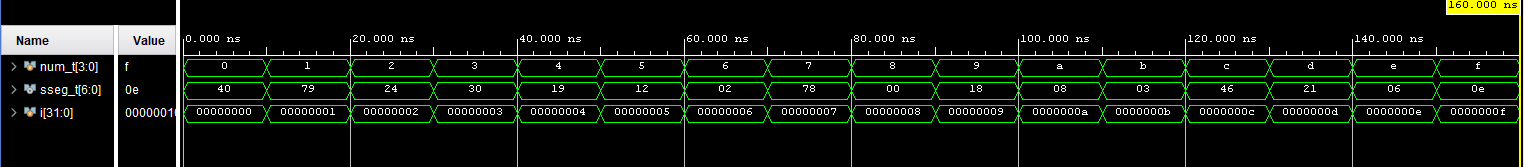
\includegraphics[width=1\textwidth]{sseg_decoder_simulation}
		\caption{the simulation waveform and ERT of the Seven-segment Decoder}
		\label{fig:sseg_decoder_simulation}
	\end{figure}
	
	Firgure 3 is the simulation waveform and ERT of the Top-level Module.
	\begin{figure}[ht]\centering
		\begin{tabular}{l|rrrr|rrrr|rrrr}
			Time (ns): & 0 & 10 & 20 & 30 & 150 & 160 & 170 & 180 & 290 & 300 & 310 & 320\\
			\midrule
			sw & 0000 & 0040 & 8040 & 0079 & 0078 & 8078 & 0000 & 8000 & 0006 & 8006 & 000e & 800e \\
			\midrule
			an & 11 & 11 & 11 & 11 & 11 & 11 & 11 & 11 & 11 & 11 & 11 & 11\\
			sseg & 40 & 40 & 19 & 18 & 00 & 78 & 40 & 40 & 02 & 40 & 06 & 40 \\
			dp & 1 & 1 & 1 & 1 & 1 & 1 & 1 & 1 & 1 & 1 & 1 & 1 \\
			an1 & 1 & 1 & 0 & 1 & 1 & 0 & 1 & 0 & 1 & 0 & 1 & 0 \\
			an0 & 0 & 0 & 1 & 0 & 0 & 1 & 0 & 1 & 0 & 1 & 0 & 1 \\
			\bottomrule
		\end{tabular}\medskip
		
		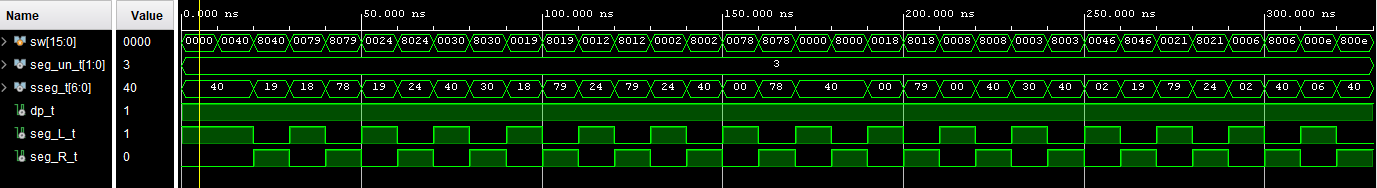
\includegraphics[width=1.1\textwidth]{sseg1_simulation}
		\caption{the simulation waveform and ERT of the Top-level Module}
		\label{fig:sseg1}
	\end{figure}
	
	This is the picture of my board which showing a value on the first digit\\
	\begin{center}
		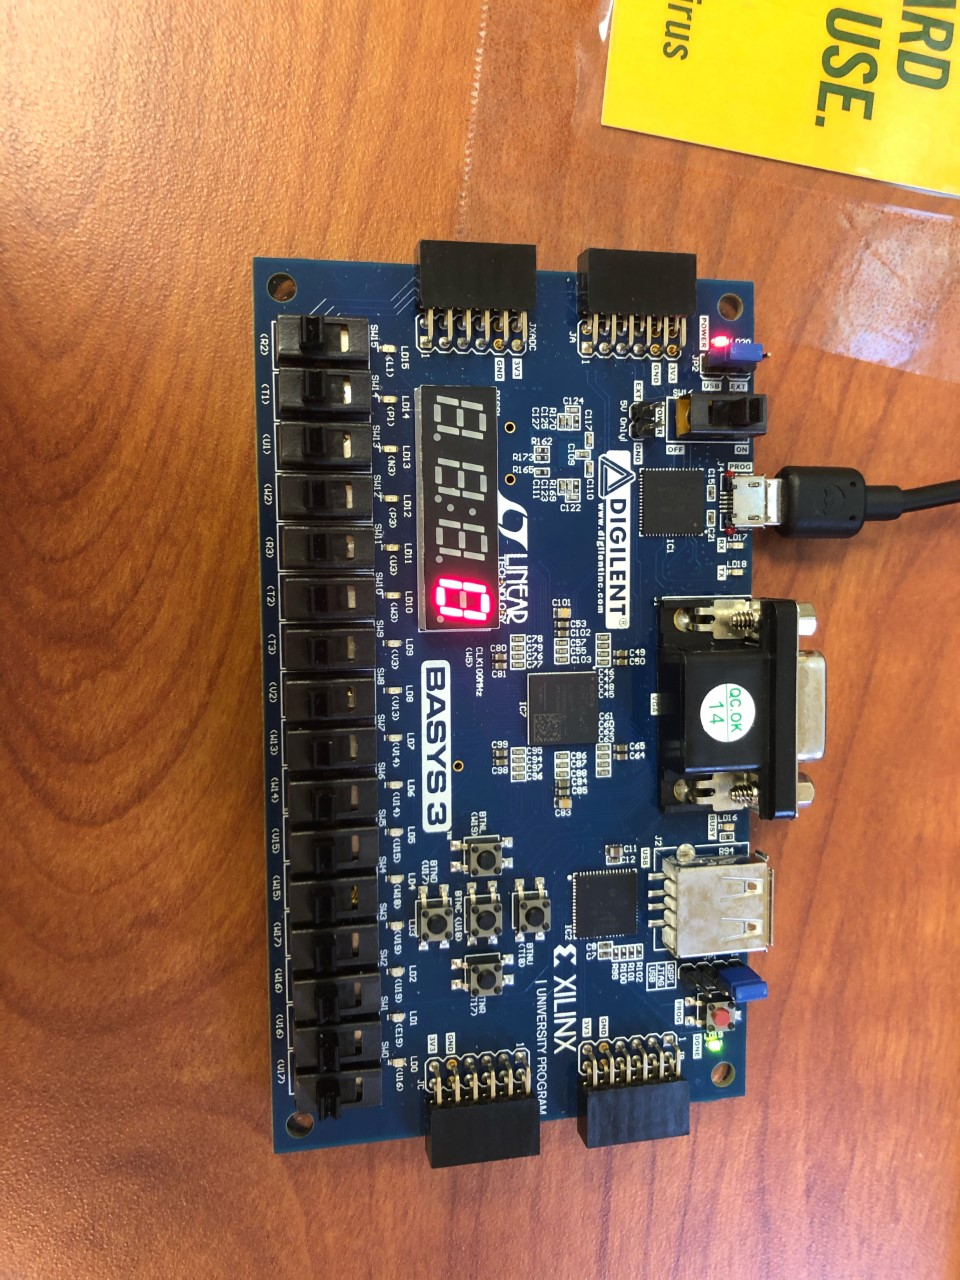
\includegraphics[width=0.5\textwidth]{board_picture1}
	\end{center}
	
	This is the picture of my board which showing a value on the second digit\\	
	\begin{center}
		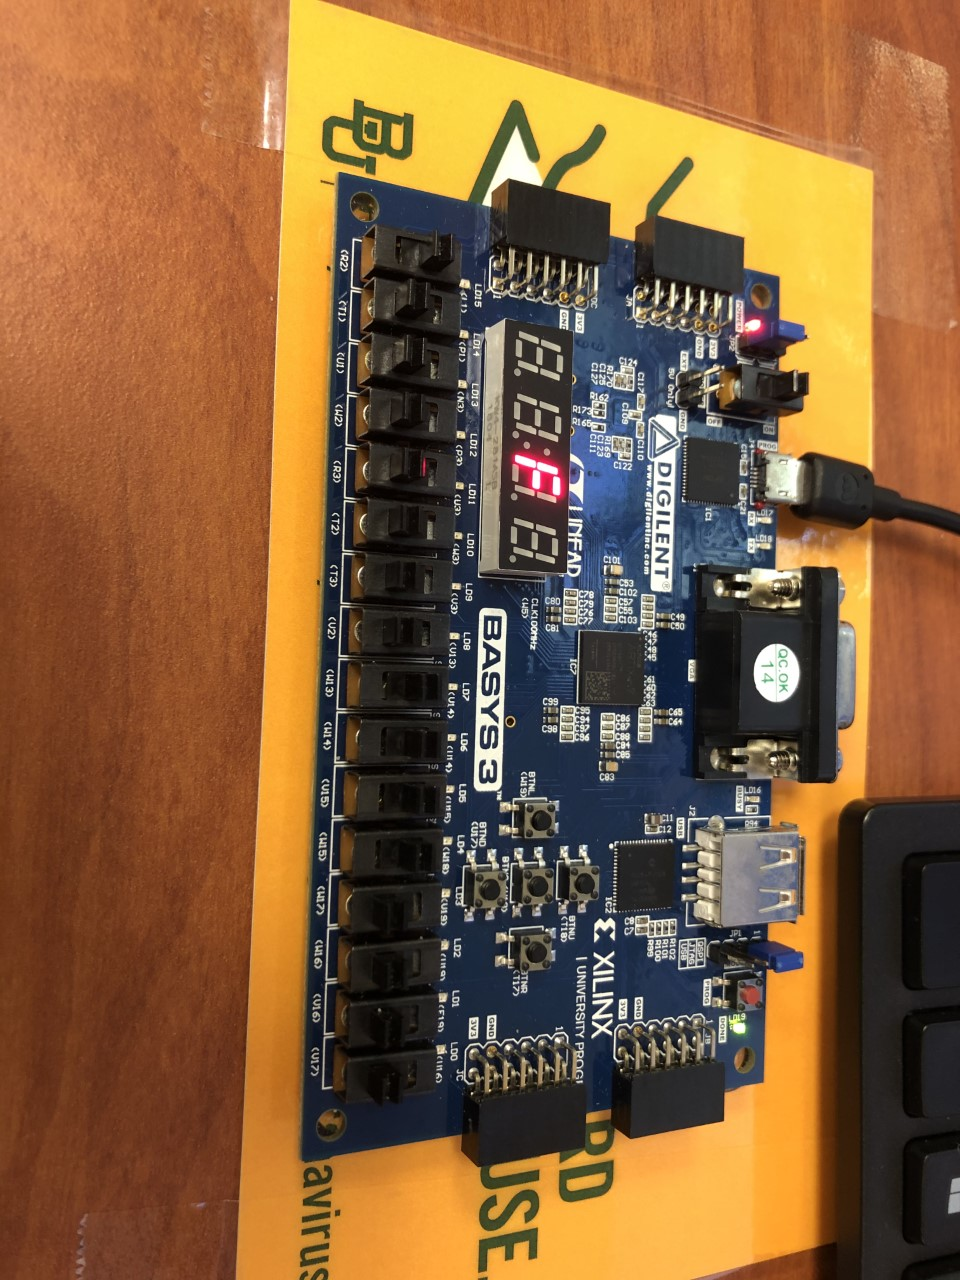
\includegraphics[width=0.5\textwidth]{board_picture2}
	\end{center}



\section*{Code}

my Verilog source file for the 4-bit Multiplexer.\\
\subsection*{File Inclusion}
\Verilog[caption=4-bit Multiplexer Verilog code,label=code:file_ex]{mux2_4b.sv}
my Verilog source file for the 4-bit Multiplexer test.\\
\subsection*{File Inclusion}
\Verilog[caption=4-bit Multiplexer Test Benches Verilog code,label=code:file_ex]{mux2_4b_test.sv}

my Verilog source file for the Seven-segment Decoder.\\
\subsection*{File Inclusion}
\Verilog[caption=Seven-segment Decoder Verilog code,label=code:file_ex]{sseg_decoder.sv}
my Verilog source file for the Seven-segment Decoder test.\\
\subsection*{File Inclusion}
\Verilog[caption=Seven-segment Decoder Test Benches Verilog code,label=code:file_ex]{sseg_decoder_test.sv}

my Verilog source file for the Top-level Module.\\
\subsection*{File Inclusion}
\Verilog[caption=Top-level Module Verilog code,label=code:file_ex]{sseg1.sv}
my Verilog source file for the Top-level Module test.\\
\subsection*{File Inclusion}
\Verilog[caption=Top-level Module Test Benches Verilog code,label=code:file_ex]{sseg1_test.sv}


\subsection*{File Inclusion}
\Verilog[caption=Two Bit Adder/Aubtractor Verilog code,label=code:file_ex]{sseg1_wrapper.sv}



\end{document}
